\section{Introduction}
\label{sec:introduction}

LLM agents are extending task execution toward proactive assistance that identifies service opportunities from ongoing observations and accumulated history.
In activity support, smart homes, and software collaboration, useful assistance depends on recognizing new needs, selecting relevant historical evidence, and tracking prior assistance.

Existing work develops proactive decisions and agent memory.
ProactiveAgent learns task proposals from activity contexts~\citep{lu2025proactiveagent}; ContextAgent combines sensed context with historical personas~\citep{yang2025contextagent}.
Mem0 consolidates and retrieves information~\citep{chhikara2025mem0}, while A-MEM links historical notes~\citep{xu2025amem}.
ProactiveBench and ContextAgentBench evaluate task proposals and contextual service; LoCoMo and LongMemEval assess long-term conversational memory~\citep{maharana2024locomo,wu2025longmemeval}.
Continuous assistance also requires assessing memory accumulation, current applicability, and changing opportunities within one event stream.
This raises a central question: \emph{how can history become source-grounded, historically supported, and currently applicable memory for timely, selective assistance?}

To study this question, we construct \emph{ProactiveStream}, a longitudinal event-stream benchmark spanning Sports, Home, and Code.
Agents build memory chronologically within isolated participant, home, and repository streams, assessing each opportunity's first actionable window and subsequent changes.
With a shared backbone and intervention control policy, existing methods show different trade-offs between opportunity recovery and false interventions (Table~\ref{tab:main_results}).
Figure~\ref{fig:intro_scenario} links earlier evening walks to current assistance.

\begin{figure}[!b]
    \centering
    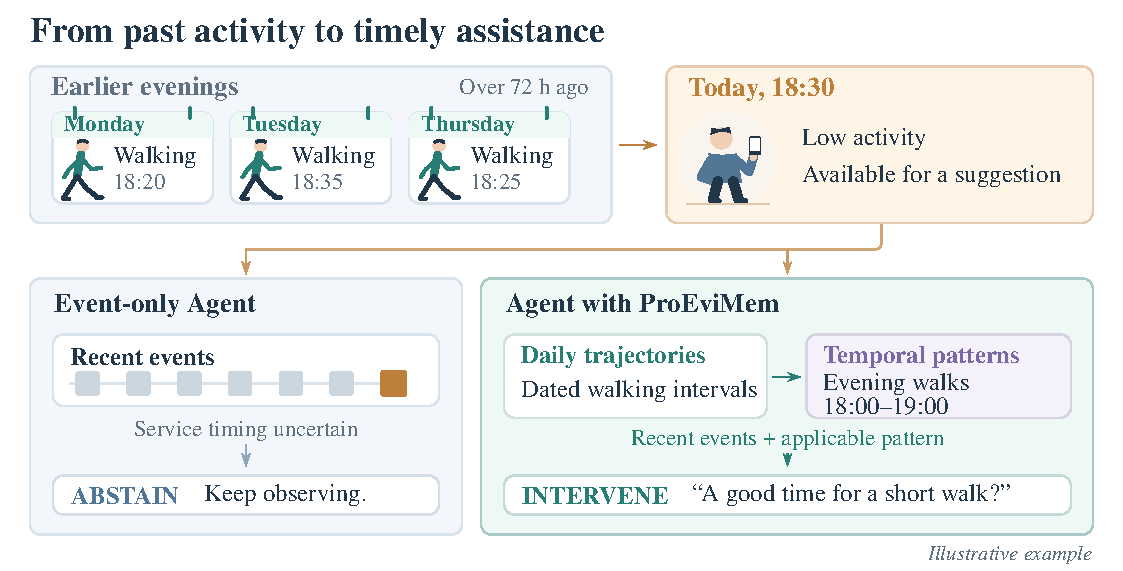
\includegraphics[width=0.96\columnwidth]{Fig_Intro_Scenario.pdf}
    \caption{Illustrative Sports scenario. \system{} retrieves a supported evening-walk regularity to guide assistance beyond recent events.}
    \label{fig:intro_scenario}
\end{figure}

We propose Proactive Memory (\system{}; Figure~\ref{fig:architecture}), linking recent observations, temporal activities, and recurring behavior.
Event memory preserves recent evidence; temporal trajectory memory abstracts source-grounded activities; behavioral regularity memory captures supported conditional behavior.
Together, these layers connect immediate changes with long-term context.

LLMs construct cited trajectories from completed events, followed by source validation of typed facts.
Historical replay assesses regularities inferred from these trajectories.
At decision time, semantic screening uses memory relevance and event-local abstention evidence to route the event.
Full assessment combines recent events, trajectories, and applicable regularities to judge service value.
Intervention control filters repeated proposals; the finalized decision precedes event commitment and memory updates.

Our contributions are:
\begin{itemize}[leftmargin=*, itemsep=0pt]
    \item ProactiveStream supports longitudinal evaluation of memory formation and repeated service decisions, preserving causal history, entity isolation, and episode-aware reference opportunities across three scopes.
    \item \system{} combines source-checked trajectory abstraction, replay-based regularity assessment, and selection of currently applicable regularities to supply historical context for proactive service decisions.
    \item \system{} uses long-term behavioral context to identify service opportunities missed by recent events alone and support more selective intervention decisions.
\end{itemize}
